\chapter{Дейтрон-протонные взаимодействия
  с перезарядкой}
В конце 1950 года на собрании Американского физического общества в
Калифорнийском Университете состоялся доклад Кладиса и его
группы~\cite{cladis50}, в котором обсуждались результаты облучения ядер дейтерия
нейтронным пучком с энергией 270 МэВ. Данные этого эксперимента были получены
на ускорителе в Беркли (США) и позднее опубликованы в
работах~\cite{cladis52,moyer52}. В докладе отмечалось, что выход быстрых
вторичных протонов (с приблизительно такой же энергией, как энергия падающих
нейтронов) в $nd$-рассеянии, в направлении падающих нейтронов, был подавлен
относительно их выхода в $np$-рассеянии в согласии с принципом Паули для двух
нейтронов с малыми относительными импульсами в реакциях с обменом заряда.

Данное экспериментальное наблюдение дало начало более детальным теоретическим
рассмотрениям, которые продолжаются и по сей день. Одним из первых в 1951 году
опубликовал свою работу Померанчук~\cite{pom51}.  В ней он указал на
возможность выяснения зависимости обменных сил от спина из сравнения процессов
рассеяния нуклонов на дейтроне с упругим рассеянием нейтрона на протоне, в
случае, когда нейтрон и протон обмениваются между собой зарядом (перезарядка). В
конце того же года, практически одновременно и независимо, с аналогичным
предложением выступил и Чу~\cite{chew51}, рассматривавший неупругое рассеяние
нейтронов на дейтроне при энергиях 90 МэВ.

Об изменении (повороте) спина одного из нуклонов в процессе $np$-перезарядки
говорилось и в работе Мигдала~\cite{mig55}. В 1957 году вышла работа
Лапидуса~\cite{lap57}, в которой обсуждалась теория обменных столкновений
быстрых нуклонов с дейтронами. В ней было показано, что сопоставление
экспериментальных данных об обменном рассеянии быстрых нуклонов дейтронами с
расчётами в импульсном приближении помогает фазовому анализу данных об
$np$-рассеянии. Автор при этом опирался на экспериментальные данные, полученные
группой Джелепова при энергиях от 380 по 590 МэВ на синхроциклотроне ИЯП АН
СССР, теперь ЛЯП ОИЯИ (измерения происходили в 1952--1954 годах, ещё до
основания Объединённого института ядерных
исследований)~\cite{dzelep56,dzelep58}.

В дальнейшем наиболее чёткая теоретическая формулировка для проведения оценки
вкладов спин-зависящей и спин-независящей частей амплитуды $np$-рассеяния из
процесса перезарядки на дейтроне была представлена в работах
Дина~\cite{dean72,dean72_2}. Полученные им формулы, выведенные в импульсном
приближении, используются во многих работах до последнего времени. Заметный
вклад в теоретический формализм и интерпретацию экспериментальных данных внесли
тоже Багг, Вилкин, Легар и другие известные учёные, теоретики.

Рассмотрим в простейшем виде два процесса, схематически изображённые на
рис.~\ref{fig:np_dp_scheme}, т.е. элементарную реакцию перезарядки нейтрона на
протоне \np и реакцию перезарядки дейтрона на протоне-мишени \dpchex. Здесь в
скобках два протона, связанные с падающим дейтроном, а именно,
протон-спектатор и протон от квази \np перезарядки, т.е. перезарядки
нейтрона (связанного в дейтроне) на протоне-мишени. Вертикальными стрелками
обозначены направления спинов нуклонов относительно произвольной оси
квантования. В первом случае, реакция \np на рис.~\ref{fig:np_dp_scheme}~а),
возможны оба направления спина рассеянного протона. Для второго случая, реакция
\dpchex на рис.~\ref{fig:np_dp_scheme}~б), при рассеянии на малый угол
(пространственная симметрия) в силу возникшей зарядовой симметрии (два протона
вылетают вперёд с малым относительным импульсом) процесс в силу принципа Паули
(статистика Ферми"--~Дирака для полуцелых спинов) может идти только с
переворотом спина у рассеянного протона. Дейтрон в данном случае выступает как
<<спиновый фильтр>>.

\begin{figure}[h]
  \centering
  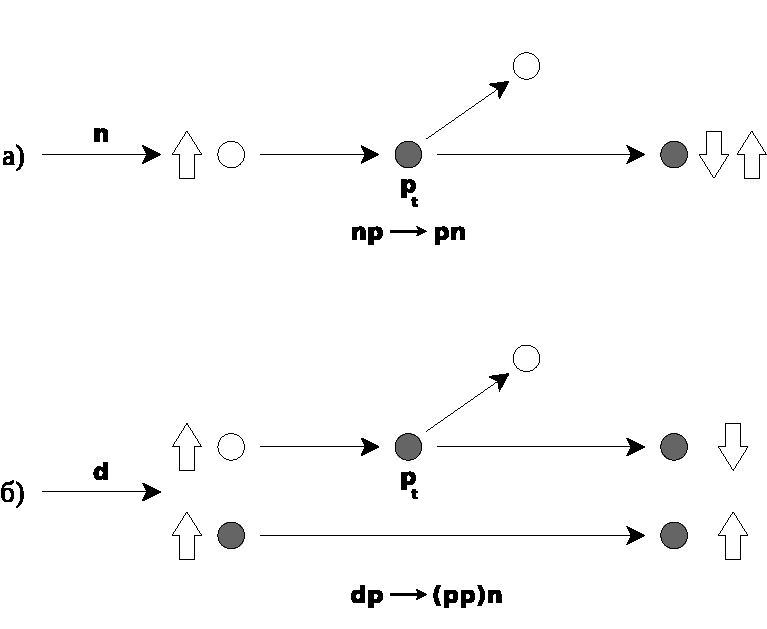
\includegraphics[width=0.85\textwidth]{np_dp_scheme.pdf}
  \caption{Схематическое изображение а) элементарной реакции перезарядки \np
    и б) перезарядки дейтрона на протоне-мишени \dpchex. Пустые кружки
    представляют нейтрон а сплошные протон, $p_{t}$~--- протон-мишени,
    вертикальные стрелки~--- направления спинов нуклонов.}
  \label{fig:np_dp_scheme}
\end{figure}

Возможность использования реакции перезарядки на дейтроне для получения
информации о спиновой зависимости реакции перезарядки \np качественно можно
объяснить следующим образом. Два нуклона~--- протон и нейтрон, связанные в
дейтроне, могут находиться в состояниях $^3S_1$ и $^3D_1$ (изоспин $I=0$)
симметричных по пространственным и спиновым переменным, но одновременно
антисимметричных по зарядовой переменной. В процессе перезарядки дейтрона на
протоне, когда образуется симметричная по заряду система из двух протонов, в
силу принципа Паули при сохранении пространственной симметрии, асимметрия полной
волновой функции дейтрона будет обеспечена переворотом спина рассеянного нуклона
(состояния $^1S_0$ или $^1D_2$ для пары протонов). Таким образом, спин-зависящая
часть амплитуды элементарной $np$-перезарядки будет проявляться через
вероятность реакции перезарядки на дейтроне~\cite{gla_mucha00}.

\section{Теоретический формализм}
\label{section:theory}
Наиболее прямым феноменологическим способом описания процесса рассеяния двух
нуклонов является определение (получение) соответствующих элементов матрицы
рассеяния непосредственно по экспериментальным данным. В описании матрицы будем
опираться на представления амплитуд нуклон-нуклонного рассеяния
Гольдбергера"--~Ватсона~\cite{gold66}. Заметим, что во многих других работах
часто используется и представление Быстрицкого, Легара,
Винтерница~\cite{bys78_2}. Оба представления амплитуд матрицы рассеяния
равнозначны и дают одинаковые результаты.

Для теоретического описания процесса нуклон-нуклонного рассеяния удобно
использовать систему центра масс с базисными векторами $(\mathbf{l, m, n})$,
определяющими ортонормированную систему координат, связанную с налетающей
частицей, где
\begin{equation}
  \label{eq:ort}
  \mathbf{l} =
  \frac{\mathbf{p}_f + \mathbf{p}_i}{|\mathbf{p}_f + \mathbf{p}_i|}\,, \qquad
  \mathbf{m} =
  \frac{\mathbf{p}_f - \mathbf{p}_i}{|\mathbf{p}_f - \mathbf{p}_i|}\,, \qquad
  \mathbf{n} =
  \frac{\mathbf{p}_i \times \mathbf{p}_f}{|\mathbf{p}_i \times \mathbf{p}_f|}\,.
\end{equation}
Векторы импульса налетающего и рассеянного нуклона обозначены $\mathbf{p}_i$ и
$\mathbf{p}_f$, соответственно. Ось базисного вектора $\mathbf{n}$
перпендикулярна к плоскости рассеяния, определённой векторами импульсов
налетающего $\mathbf{p}_i$ и рассеянного $\mathbf{p}_f$ нуклона.

В общем виде, матрицу рассеяния $T$, феноменологически описывающую процесс
$NN$-рассеяния, можно записать с помощью линейных функций $A$ и $B$, зависимых
от $\boldsymbol{\sigma}_1$ и трёх ортогональных векторов, определённых
выражением~\eqref{eq:ort}, в виде
\begin{equation}
  \label{eq:mat}
  T = A + B\,\boldsymbol{\sigma}_2\,,
\end{equation}
где $\boldsymbol{\sigma}_1$ и $\boldsymbol{\sigma}_2$~--- $2 \times 2$-спиновые
матрицы Паули действующие на волновую функцию налетающего нуклона и
нуклона-мишени. При разложении функций $A$ и $B$ по объединённому спиновому
пространству обоих нуклонов матрица рассеяния~\eqref{eq:mat} имеет следующий
общий вид
\begin{equation}
  \label{eq:mat_full}
  \begin{split}
    T = \ &\ a_1 +
    a_2(\boldsymbol{\sigma}_1\cdot\mathbf{l}) +
    a_3(\boldsymbol{\sigma}_1\cdot\mathbf{m}) +
    a_4(\boldsymbol{\sigma}_1\cdot\mathbf{n})\ + \\
    +\ &\bigl[b_1 +
      b_2(\boldsymbol{\sigma}_1\cdot\mathbf{l}) +
      b_3(\boldsymbol{\sigma}_1\cdot\mathbf{m}) +
      b_4(\boldsymbol{\sigma}_1\cdot\mathbf{n})\bigr]
    \,(\boldsymbol{\sigma}_2\cdot\mathbf{l})\ + \\
    +\ &\bigl[c_1 +
      c_2(\boldsymbol{\sigma}_1\cdot\mathbf{l})\,+
      c_3(\boldsymbol{\sigma}_1\cdot\mathbf{m}) +
      c_4(\boldsymbol{\sigma}_1\cdot\mathbf{n})\bigr]
    \,(\boldsymbol{\sigma}_2\cdot\mathbf{m})\ +\\
    +\ &\bigl[d_1 +
      d_2(\boldsymbol{\sigma}_1\cdot\mathbf{l}) +
      d_3(\boldsymbol{\sigma}_1\cdot\mathbf{m}) +
      d_4(\boldsymbol{\sigma}_1\cdot\mathbf{n})\bigr]
    \,(\boldsymbol{\sigma}_2\cdot\mathbf{n})\,,
  \end{split}
\end{equation}
где коэффициенты $a_i, b_i, c_i$ и $d_i$ относятся к комплексным амплитудам
нуклон-нуклонного рассеяния. Спиновая матрица размером
$4 \times 4$~\eqref{eq:mat_full} полностью описывает всю динамику процесса
рассеяния двух нуклонов.

Следуя работе~\cite{gold66}, все 16 матричных элементов можно выразить через 5
амплитуд рассеяния, если наложить требования пространственной и временной
инвариантности, а также предполагать зарядовую симметрию ядерных сил. Такие
предположения позволяют представить общий вид матрицы рассеяния $T$ в упрощённой
форме
\begin{equation}
  \label{eq:mat_final}
  \begin{split}
    T =\ &a\ +\ b
    (\boldsymbol{\sigma}_1\cdot\mathbf{n})
    (\boldsymbol{\sigma}_2\cdot\mathbf{n})\ +\ c\bigl[
      (\boldsymbol{\sigma}_1\cdot\mathbf{n}) +
      (\boldsymbol{\sigma}_2\cdot\mathbf{n})\bigr]\ \ +\\
    +\ &e
    (\boldsymbol{\sigma}_1\cdot\mathbf{m})
    (\boldsymbol{\sigma}_2\cdot\mathbf{m})\ +\ f
    (\boldsymbol{\sigma}_1\cdot\mathbf{l})
    (\boldsymbol{\sigma}_2\cdot\mathbf{l})\,.
  \end{split}
\end{equation}
Комплексные амплитуды $a, b, c, e$ и $f$ являются функциями энергии реакции и
угла рассеяния взаимодействующих частиц. Таким образом, нуклон-нуклонное
рассеяние в общем виде полностью описывается всего пятью комплексными
амплитудами. Из уравнения~\eqref{eq:mat_final} видно, что только первый член
матрицы рассеяния $T$, комплексная амплитуда $a$, не зависит от спина.

Дифференциальное поперечное сечение \np рассеяния, следуя работе~\cite{bys78_2},
можно записать как
\begin{equation}
  (d\sigma/dt)_{\np} = (\pi/p^2)\,
  \bigl[\,|a|^2 + |b|^2 + 2|c|^2 + |e|^2 + |f|^2 \bigr]
\end{equation}
и может быть представлено в виде суммы спин-независящей (индекс $SI$) и
спин-зависящей (индекс $SD$) частей
\begin{equation}
  (d\sigma/dt)_{\np} = (d\sigma/dt)^{SI}_{\np} + (d\sigma/dt)^{SD}_{\np}\,,
\end{equation}
где $p$~--- импульс с системе центра масс двух нуклонов, а $t$~--- квадрат
четырёхмерного переданного импульса. Для отдельных частей дифференциального
сечения получаем
\begin{align}
  (d\sigma/dt)^{SI}_{\np} &= (\pi/p^2)\,|a|^2\,,\\
  \label{eq:np_SD}
  (d\sigma/dt)^{SD}_{\np} &= (\pi/p^2)\,
  \bigl[\,|b|^2 + 2|c|^2 + |e|^2 + |f|^2\bigr]\,.
\end{align}

Математический формализм, который в рамках импульсного приближения позволяет
записать дифференциальное поперечное сечение реакции перезарядки на дейтроне
через дифференциальное поперечное сечение элементарной реакции перезарядки
на нуклоне, обсуждался во многих работах~\cite{dean72,dean72_2,bugg87}.
В импульсном приближении, амплитуда рассеяния нуклонов сложным ядром (дейтроном)
представляется в виде суммы амплитуд рассеяния свободными нуклонами, имеющими
распределение импульсов, соответствующее в данный момент распределению импульсов
нуклонов в ядре~\cite{chew50,chew52}. Рассеяние падающей частицы на ядре можно
потом приблизительно рассматривать, как происходящее на отдельных нуклонах, так
как энергия связи частиц в ядре играет второстепенную роль, особенно в случае
дейтрона.

Соотношение между дифференциальными поперечными сечениями перезарядки дейтрона
на протоне \dpchex и элементарной перезарядкой \np при применении импульсного
приближения можно записать~\cite{dean72_2} как
\begin{equation}
  (d\sigma/dt)_{\dpchex} = \bigl[1 - F_d(t)\bigr]\,(d\sigma/dt)^{SI}_{\np} +\,
  \bigl[1 - 1/3\,F_d(t)\bigr]\,(d\sigma/dt)^{SD}_{\np}\,,
\end{equation}
где $F_d(t)$ обозначает формфактор дейтрона. Из этой формулы следует, что при
нулевой передаче импульса $(t=0)$, из-за того, что $F_d(0) = 1$,
дифференциальное поперечное сечение будет иметь следующий вид
\begin{equation}
  \label{eq:dp_23np}
  (d\sigma/dt)_{\dpchex} = 2/3\,(d\sigma/dt)^{SD}_{\np}\,.
\end{equation}

Таким образом, появилась возможность определения части взаимодействия нейтрона и
протона, которая полностью зависит от спина, из экспериментального анализа
дифференциального сечения реакции перезарядки дейтрона на протоне \dpchex ,
используя данные по перезарядке в элементарном процессе \np на неполяризованном
пучке и неполяризованном протоне-мишени.

Мы рассматриваем случай рассеяния назад, когда угол двух рассеявшихся нуклонов
(нейтрона и протона) близок к 180$^{\,\circ}$. При этих условиях вектор импульса
налетающего нуклона антипараллелен вектору импульса рассеянного нуклона
$(\mathbf{p}_i = -\,\mathbf{p}_f)$, а для амплитуд рассеяния выполняется
соотношение $b(\pi) = f(\pi)$ и $c(\pi) = 0$.  В итоге, следуя
уравнениям~\eqref{eq:np_SD} и~\eqref{eq:dp_23np}, для дифференциального
поперечного сечения \np рассеяния назад получаем простое выражение
\begin{equation}
  (d\sigma/dt)_{\dpchex} = 2/3\,(d\sigma/dt)^{SD}_{\np} =
  2/3\,(\pi/p^2)\,\bigl[\,2\,|b|^2 + |e|^2\bigr]\,.
\end{equation}
Изучение процесса перезарядки \dpchex при нулевых переданных импульсах позволяет
оценить спин-зависящую часть сечения элементарной реакции перезарядки \np,
которая определяется суммой всего двух амплитуд $2\,|b|^2 + |e|^2$.

\section{Сечение реакции перезарядки \maybebm{{\np}}}
\label{section:npnp}
Как видно из вышесказанного, для того, чтобы сделать оценку вклада
спин-зависящей части амплитуды \np рассеяния, используя данные по реакции
перезарядки на дейтроне, необходимо, кроме измерения дифференциального
поперечного сечения реакции \dpchex, иметь данные экспериментов по
дифференциальному сечению реакции элементарной перезарядки \np при $t=0$.
Из наших экспериментальных данных, которые были получены в пучке дейтронов
импульса 3.35~ГэВ/с, мы будем оценивать величину дифференциального поперечного
сечения для перезарядки на дейтроне при $t=0$ и сравниваем её с имеющимися в
литературе данными по этой величине для \np рассеяния при том же импульсе.

В работе Фридеса и др.~\cite{friedes65} проведённой в Брукхейвене (США) были
просуммированы данные по дифференциальному сечению реакции \np в диапазоне
импульсов нейтронов от 1.4 до 8.15~ГэВ/с и приведена полученная авторами
зависимость $d\sigma/dt\,|\,_{t=0}$ от импульса (более детальная информация об
этих измерениях отсутствует). Известна также работа Шепарда и др.~\cite{shep69},
позднее опубликованная в~\cite{shep74} по перезарядке в $np$-рассеянии в
диапазоне импульсов 600--2000 МэВ/с на протонном ускорителе в Принстоне (США).

Как и в других подобных экспериментах, пучок вторичных нейтронов формировался от
взаимодействий ускоренных протонов на внутренней мишени ускорителя. С помощью
магнитов, отклоняющих вторичные заряженные частицы, и коллиматоров пучок
нейтронов направлялся на жидководородную мишень. Выходящие из мишени в переднем
направлении быстрые протоны анализировались магнитным спектрометром.

Позднее на ускорителе Сатурн в Сакле (Франция) были проведены Бизардом и
др. систематические измерения дифференциальных сечений реакции перезарядки \np в
интересующем нас диапазоне импульсов нейтронов 1--2 ГэВ/с~\cite{biz75}. В
отличие от других аналогичных экспериментов, в этой работе использовались
квази-монохроматические нейтроны от стриппинга ускоренных дейтронов с импульсным
разбросом 5~$\%$.

Последний из нам известных экспериментов по $np$-рассеянию в интересующем нас
диапазоне энергий и с результатами по дифференциальному сечению при малых
значениях $t$ был выполнен в лаборатории Лос Аламос~(США) и опубликован в работе
Боннера и др.~\cite{bon78}.

На основе экспериментальных данных этих цитируемых работ, для каждого значения
импульса нейтрона в интервале от 1 до 2~ГэВ/с, строилась зависимость
дифференциального поперечного сечения $d\sigma/dt$ элементарной реакции
перезарядки \np от четырёхмерного переданного импульса $t$. На
рис.~\ref{fig:np_two_bizard} в качестве примера приведена такая зависимость для
двух разных импульсов налетающего нейтрона (измерения на ускорителе Сатурн при
импульсе 1.43 и 1.88 ГэВ/с).

\begin{figure}[h]
  \centering
  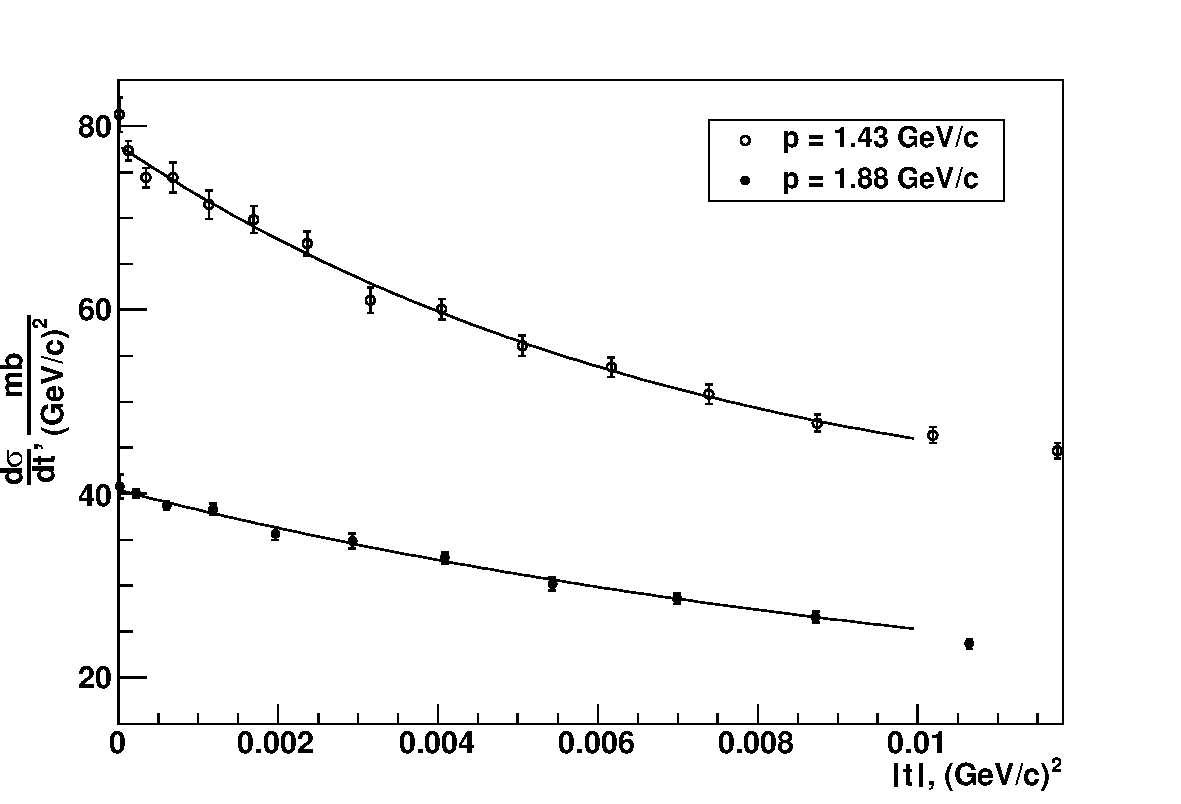
\includegraphics[width=1.00\textwidth]{np_two_bizard.pdf}
  \caption{Зависимость дифференциального поперечного сечения $d\sigma/dt$
    реакции перезарядки \np от четырёхмерного переданного импульса $t$ для двух
    разных импульсов $p$ налетающего нейтрона. Сплошные линии~--- аппроксимация
    экспериментальных данных функцией \eqref{eq:exp2}.}
  \label{fig:np_two_bizard}
\end{figure}

Индивидуальные сечения $d\sigma/dt$ при $t=0$ были получены путём аппроксимации
распределений $d\sigma/dt$ для каждого (всего~39) значения импульса нейтрона
выражением
\begin{equation} \label{eq:exp2}
  d\sigma/dt = p_0\exp(p_1\,t + p_2\,t^2)
\end{equation}
в интервале $t < 0.01$~(ГэВ/с)$^2$ и затем экстраполировались в точку $t=0$.
Полученные дифференциальные поперечные сечения $d\sigma/dt\,|\,_{t=0}$ реакции
перезарядки \np в интервале импульсов от 1 до 2~ГэВ/с приведены в
таблице~\ref{tab:np_data} и на рис.~\ref{fig:np_sigma0}.

\begin{table}[hp]
  \begin{center}
    \bigskip
    \resizebox{1.0\textwidth}{!} {
      \begin{tabular}{|c|c|c|}
        \hline $p$\,, & $d\sigma/dt\,|\,_{t=0}$\,, & Лаб. \\
        ГэВ/с & (ГэВ/с)$^2$ & \\ \hline \hline
        1.025 & 152.219 $\pm$ 0.873 & Лос Аламос \\ \hline
        1.033 & 156.199 $\pm$ 1.646 & Сакле \\ \hline
        1.045 & 144.949 $\pm$ 3.795 & Принстон \\ \hline
        1.055 & 142.571 $\pm$ 0.763 & Лос Аламос \\ \hline
        1.083 & 134.839 $\pm$ 1.310 & Сакле \\ \hline
        1.085 & 136.435 $\pm$ 0.571 & Лос Аламос \\ \hline
        1.115 & 129.173 $\pm$ 0.534 & Лос Аламос \\ \hline
        1.132 & 124.928 $\pm$ 1.150 & Сакле \\ \hline
        1.145 & 120.877 $\pm$ 0.594 & Лос Аламос \\ \hline
        1.146 & 114.784 $\pm$ 4.271 & Принстон \\ \hline
        1.175 & 115.738 $\pm$ 0.584 & Лос Аламос \\ \hline
        1.182 & 109.973 $\pm$ 0.958 & Сакле \\ \hline
        1.205 & 107.189 $\pm$ 0.650 & Лос Аламос \\ \hline
        1.232 & 105.913 $\pm$ 1.080 & Сакле \\ \hline
        1.235 & 101.102 $\pm$ 0.691 & Лос Аламос \\ \hline
        1.260 & 98.797 $\pm$ 0.750 & Лос Аламос \\ \hline
        1.281 & 74.825 $\pm$ 2.804 & Принстон \\ \hline
        1.281 & 86.811 $\pm$ 1.332 & Сакле \\ \hline
        1.295 & 92.099 $\pm$ 0.735 & Лос Аламос \\ \hline
        \multicolumn{3}{|r|}{{продолжение \dots}} \\ \hline
      \end{tabular}
      \quad
      \begin{tabular}{|c|c|c|}
        \hline $p$\,, & $d\sigma/dt\,|\,_{t=0}$\,, & Лаб. \\
        ГэВ/с & (ГэВ/с)$^2$ & \\ \hline \hline
        1.325 & 86.636 $\pm$ 0.687 & Лос Аламос \\ \hline
        1.331 & 87.610 $\pm$ 1.148 & Сакле \\ \hline
        1.355 & 85.586 $\pm$ 0.700 & Лос Аламос \\ \hline
        1.381 & 77.721 $\pm$ 0.721 & Сакле \\ \hline
        1.385 & 81.942 $\pm$ 0.612 & Лос Аламос \\ \hline
        1.429 & 73.384 $\pm$ 0.303 & Лос Аламос \\ \hline
        1.431 & 77.932 $\pm$ 0.694 & Сакле \\ \hline
        1.481 & 68.842 $\pm$ 0.699 & Сакле \\ \hline
        1.484 & 53.359 $\pm$ 2.384 & Принстон \\ \hline
        1.531 & 70.749 $\pm$ 0.983 & Сакле \\ \hline
        1.580 & 59.855 $\pm$ 1.235 & Сакле \\ \hline
        1.630 & 56.144 $\pm$ 1.172 & Сакле \\ \hline
        1.680 & 59.372 $\pm$ 0.846 & Сакле \\ \hline
        1.729 & 40.091 $\pm$ 1.962 & Принстон \\ \hline
        1.730 & 53.252 $\pm$ 0.584 & Сакле \\ \hline
        1.780 & 47.591 $\pm$ 0.434 & Сакле \\ \hline
        1.831 & 43.857 $\pm$ 0.401 & Сакле \\ \hline
        1.881 & 40.405 $\pm$ 0.391 & Сакле \\ \hline
        1.931 & 35.176 $\pm$ 0.507 & Сакле \\ \hline
        1.981 & 28.170 $\pm$ 0.675 & Сакле \\ \hline
      \end{tabular}
    }
    \bigskip
    \caption{Дифференциальные поперечные сечения $d\sigma/dt\,|\,_{t=0}$ для
      реакции элементарной перезарядки \np в интервале импульсов от 1 до 2
      ГэВ/с. Значения сечений получены на основе экспериментальных данных
      лабораторий Лос Аламоса~\cite{bon78}, Сакле~\cite{biz75} и Принстонского
      университета~\cite{shep74}.}
    \label{tab:np_data}
  \end{center}
\end{table}



%%% Local Variables:
%%% mode: latex
%%% TeX-master: "../musinsky_disser"
%%% coding: utf-8
%%% End:


\begin{figure}[h]
  \centering
  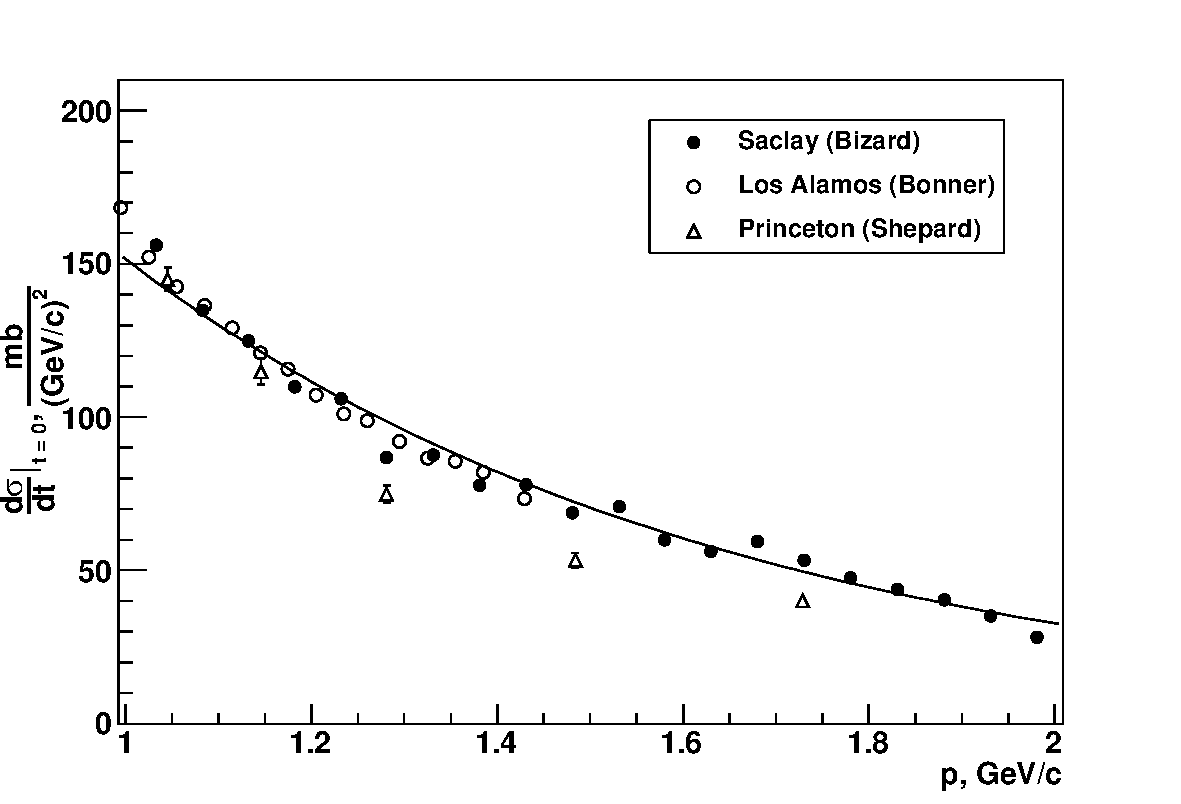
\includegraphics[width=1.00\textwidth]{np_sigma0.pdf}
  \caption{Зависимость дифференциального поперечного сечения
    $d\sigma/dt\,|\,_{t=0}$ элементарной реакции перезарядки \np от импульса $p$
    налетающего нейтрона. Сплошная линия~--- аппроксимация простой
    экспоненциальной функцией.}
  \label{fig:np_sigma0}
\end{figure}

Как видно, сечения перезарядки при $t=0$, полученные в Принстоне, оказались в
противоречии с данными других работ (были занижены примерно на 20~$\%$). Причина
такого расхождения неоднократно дискутировалась в научной периодике, но так и не
была объяснена. С другой стороны, данные полученные в Лос Аламосе очень близки к
данным Сакле. Поэтому считается, что измерения, проведённые Бизардом и др. на
ускорителе Сатурн в Сакле являются более корректными~\cite{biz75,bys78,nn_web}.
К тому же они проведены в интересующей нас области энергий 1 ГэВ и выше.

Зависимость, показанная на рис.~\ref{fig:np_sigma0}, была аппроксимирована
простой экспоненциальной функцией (аппроксимируются только данные получены
Бизардом и др.). В результате получаем выражение зависимости значения
$d\sigma/dt\,|\,_{t=0}$ реакции перезарядки \np от импульса $p$ налетающего
нейтрона
\begin{equation}
  \label{eq:np0}
  (d\sigma/dt\,|\,_{t=0})/p = 713.112 \exp(-1.533\,p)\,,
\end{equation}
которое будем в дальнейшем использовать.

Доступность результатов измерений, приведённых в работе Бизарда и др., дала
возможность проведения оценки спин-зависящей части амплитуды $np$-рассеяния при
их анализе совместно с результатами измерений дифференциальных сечений
перезарядки на дейтроне. Отметим, что опубликованные ранее данные~\cite{mucha02}
были сравнены с сечениями из работ Фридеса и
Шепарда~\cite{friedes65,shep69,shep74}, в которых значения
$d\sigma/dt\,|\,_{t=0}$ реакции перезарядки \np были, как было показано,
занижены.

\section{Избранные исследования с дейтронами}
В 80-х годах на синхрофазотроне ЛВЭ ОИЯИ были ускорены дейтроны, сначала с целью
получения вторичных нейтронных пучков от реакций стриппинга на бериллиевой
мишени. Был сформирован  канал в направлении на водородную камеру и в дальнейшем
она была экспонирована нейтронами нескольких энергий. Одновременно, используя
уже имевшийся канал для транспортировки заряженных частиц, камера облучалась
выведенным из ускорителя пучком дейтронов. Появилась возможность изучать
дейтрон-протонные взаимодействия с помощью водородной пузырьковой камеры в
условиях 4$\pi$-геометрии. Было получено большое количество результатов по
различным направлениям исследований и создана база данных, в частности, по
реакции перезарядки \dpchex. Результаты этого эксперимента будут обсуждены в
следующей главе диссертации.

Другой группой физиков (Струнов, Шаров) была создана установка
Дельта-Сигма~\cite{shar00}. На этой установке изучалась разница полных сечений
нейтрон-протонных взаимодействий  при двух различных направлениях продольной
поляризации падающего нейтрона и протона в поляризованной мишени. Позднее
установка была дополнена магнитным спектрометром для измерения импульсов
протонов из процессов $np$-перезарядки вылетающих в переднем направлении.

В этих работах использовались как жидководородная, так и жидкодейтериевая
мишени, что позволило в рамках одной геометрии эксперимента измерять
дифференциальные сечения как $np$, так и $nd$-процессов перезарядки. Авторам
удалось пройти в ранее неисследованную область энергий нейтронов выше
1~ГэВ. Мишень установки была окружена сцинтилляционными счётчиками работающими в
режиме антисовпадения с целью уменьшения фона от неупругих
процессов~\cite{shar04}.

Нам известно также об экспозиции водородной пузырьковой камеры в пучке
сепарированных дейтронов в KEK (Япония) в диапазоне импульсов
2.0--3.7~ГэВ/с~\cite{kata85}. Однако, в этой работе изучались только
дифференциальные сечения упругого \dpela рассеяния.

В Петербургском институте ядерной физики (ПИЯФ, Гатчина) в 80-х годах работала
жидкодейтериевая камера. В пучке протонов от синхроциклотрона ЛИЯФ АН СССР в
диапазоне импульсов от 1140 до 1426 МэВ/с изучалась~\cite{and85} реакция
$pd \rightarrow ppn$. В такой постановке опыта, где ускоренные протоны падают на
покоящиеся дейтроны, можно было регистрировать и изучать только лишь события с
быстрыми вторичными протонами, выше 80--100~МэВ/с, так как более медленные не
регистрируются в пузырьковой камере из за малого пробега. Кстати, это
обстоятельство не позволило изучать процесс перезарядки при малых переданных
импульсах. Авторы изучали только кумулятивные процессы.

В последние годы ускорение дейтронов \! было осуществлено на ускорителе COSY в
Юлихе (Германия) и на установке ANKE стал осуществляться проект по изучению
процессов перезарядки на дейтроне, в том числе и поляризованном. В
работе~\cite{chila09} приведены анализирующие способности реакции фрагментации
дейтрона, однако значения дифференциального сечения в зависимости от $t$ не
приведены.

\section{Выводы к первой главе}
Основные выводы данной главы можно сформулировать следующим образом:
\begin{list}{\labelitemi}{\leftmargin=1em}
\item Обсуждена возможность использования реакции перезарядки на
  неполяризованном дейтроне для извлечения оценки спин-зависящей части амплитуды
  \np перезарядки на основе прямого измерения дифференциального сечения.
\item Представлен математический формализм для вычисления спин-зависящей части
  амплитуды \np перезарядки исходя из измеренного значения $d\sigma/dt$ при
  $t=0$ реакции перезарядки  \dpchex и известного сечения $d\sigma/dt$  при
  $t=0$ элементарной перезарядки \np в рамках импульсного приближения.
\item Исходя из имеющихся мировых данных извлечена зависимость значения
  дифференциального поперечного сечения \np перезарядки от импульса при нулевой
  передаче четырёхимпульса.
\item Рассмотрение экспериментальных данных по определению спин-зависящей части
  амплитуды \np перезарядки показало, что в настоящее время существует более или
  менее полная картина в интервале энергий до 1~ГэВ. В области энергий выше
  1~ГэВ экспериментальная информация скудна и продолжение исследований в этой
  области энергий остаётся актуальным.
\end{list}

%%% Local Variables:
%%% mode: latex
%%% TeX-master: "musinsky_disser"
%%% coding: utf-8
%%% End:
